\section{Vorverarbeitung}
\label{sec:03_Preprocessing}
Ziel der Vorverarbeitung ist es, durch Aufbereitung der Daten, den
Informationsgehalt zu maximieren sowie Rauschen zu minimieren.
Des Weiteren müssen die Daten so vorverarbeitet werden, dass diese 
von den maschinellen Lern Algorithmen ausgewertet werden können. 

Um das Untergrund-Rauschen zu minimieren, könnten Bildausschnitte, auf 
denen keine Wolken zu erkennen sind herausgeschnitten werden.
Stattdessen wird auf die Methode der Farb-Filter zurückgegriffen, da dabei 
keine manuelle Nachbearbeitung der Fotos notwendig ist und somit ein höherer 
Automatisierungsgrad erreicht wird.

Dazu werden Bilder, die weniger als \SI{30}{\percent} der maximalen Helligkeit 
besitzen, verworfen. 
Anders als beispielsweise bei einer Zeitschaltuhr lässt sich durch die
Separation anhand des Helligkeitswert die Messzeit maximieren, da die 
Belichtung sowohl vom Monat als auch von der Wolkendecke abhängig ist.
Fotos welche nicht dem Helligkeits-Schnitt überstehen, werden noch bevor 
sie gelabelt werden der Klasse \texttt{schlechte Fotos} zugeordnet um 
den Arbeitsaufwand geringer zu halten.

\begin{wrapfigure}{r}{0.5\textwidth}
		\centering
		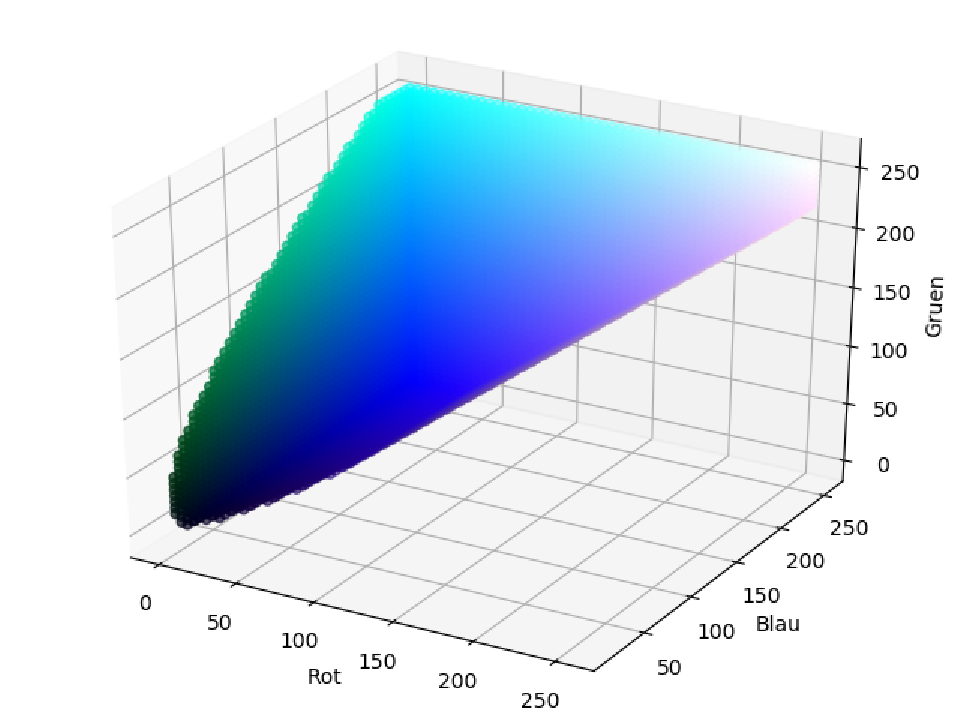
\includegraphics[width=0.49\textwidth]{pictures/cut_cube.pdf}
		\caption{Um den Winkel $\alpha$ zur grünen Ebene geneigte Parabel im RGB 
				Farbraum, welche zu den Blauwerten geöffnet ist.}
				\label{fig:parabular}
\end{wrapfigure}
Das Wolkenspektrum hat klar definierte Farben, das hauptsächlich aus Blau, Grau
und Weiß Tönen besteht.
Pixel, die nicht zu diesem Spektrum gehören, werden systematisch auf den
Minimalwert gesetzt.
Dazu wird der Farbraum in ein rotiertes System $RGB'$ mittels der 
Rotationsmatrix $R_{\alpha}$ um den Nullpunkt gedreht. 
In den rotierten Farbraum $RGB'$ wird eine Parabel gelegt, die Pixel
verwirft, welche die Ungleichung 
\begin{equation}
		c' > (b' - x_0)^2 + x_1, \hspace{3em} c' \in (r', g')
\end{equation}
nicht erfüllen.
Im Anschluss wird die Parabel in den unursprünglichen Raum zurück
rotiert.
Der Nullpunkt der Parabel wird mit den Helligkeitswerten verschoben.
Ein Beispiel ist für alle drei Kanäle in Abbildung \ref{fig:parabular} zu sehen.
Dadurch lässt sich ein Großteil der mitfotografierten Untergrunddaten durch
eine konstanten Wert \texttt{(0,0,0)} ersetzen.
\begin{figure}
		\centering
		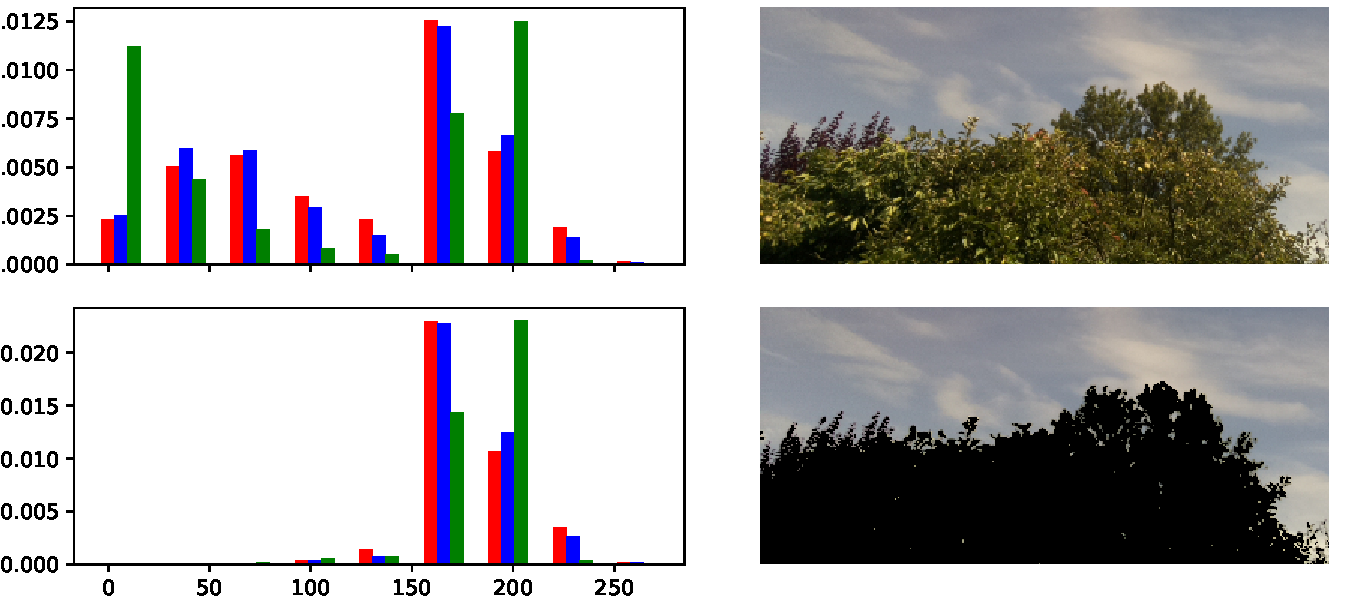
\includegraphics[width=0.95\textwidth]{pictures/cut_hist.pdf}
		\caption{Anhand des Farbspektrums geschwärzter Untergrund und die
		dazugehörigen Farbspektren zur Reduzierung des Umgebungsrauschens mit
		\texttt{bins = 10} zur Veranschauungszwecken.}
		\label{fig:name}
\end{figure}

Nachdem die Daten entsprechend aufbereitet wurden müssen sie noch in Form für
die Algorithmen gebracht werden. 
Dazu wird der Farbraum für den Random Forest diskretisiert.
Durch mehrmaliges Austesten kristallisierte sich eine Anzahl von 
\texttt{bins = 30} als die Diskretisierung mit den besten Ergebnissen heraus,
wobei die auf den konstanten Wert gesetzten Untergrunddaten kein Teil des
Histogramms sind.
Für das Neuronale Netz werden die Bilddaten auf eins normiert und mittels 
eines \texttt{ImageDataGenerator} sequentiell aus den \texttt{JPG}-Dateien 
eingelesen. 
Dadurch lässt sich das Überlaufen des begrenzten Arbeitsspeicher auf Kosten 
der Trainingszeit, durch das wiederholte Laden der Daten von der Festplatte,
verhindern.


\section{Maschinelles Lernen}

Zur automatischen Bestimmung des Wolkentyps werden zwei verschiedene 
Algorithmen verwendet. 
Der Random Forest wird verwendet, weil dieser out of-the-box hinreichend 
schnell und in der Auswertung und ressourcenschonend ist.
Des Weiteren wird ein CNN benutzt, da dieses im Gegensatz zum Random Forest in 
der Lage ist, sowohl auf den Wolkenformen, als auch auf dem 
Farbspektrum zu trainieren. 

Beim Training der Algorithmen stellte sich heraus, dass die Daten aufgrund des im
Kapitel \ref{sec:02_Datensatz} beschriebenen Problem einen großen Mismatch 
aufweisen. 
Aufgrund dessen ändert sich die Zielstellung bei der Optimierung wesentlich.
Ziel ist vorerst nicht, eine möglichst hohe Genauigkeit zu erlangen,
um die Wolkenklassifikation auf den Raspberry Pis voran zu treiben,
sondern nun den Datensatz zu erweitern und den Mismatch zu 
minimieren.
Dazu werden die Methoden genutzt, um die Wolken, welche nicht mit dem 
aktuellen Label übereinstimmen, mittels dem \texttt{TelegramBot} erneut zu überprüfen.
Des Weiteren wird bei dem Labeln neuer Daten ein Label vorgeschlagen,
welches übernommen oder per Hand geändert werden kann.
\begin{figure}
		\centering
		\includegraphics[width=\textwidth]{build/vorgehen.pdf}
		\caption{Modell für das weitere Vorgehen zur Verbesserung der Vorhersagen
		der maschinellen Modelle durch Erstellung eines reinen Datensatzes.}
		\label{fig:}
\end{figure}

Die Metrik, anhand derer die Modelle evaluiert werden, bleibt die 
Accuracy wobei abgeleitete Größen, wie der Loss oder Confidencewerte, kritisch bei Daten welche einen Mismatch haben zu 
betrachten sind.

\subsection{Random Forest}%
\label{sub:random_forest}
\begin{wrapfigure}{r}{0.5\textwidth}
		\centering
		\vspace{-1.2cm}
		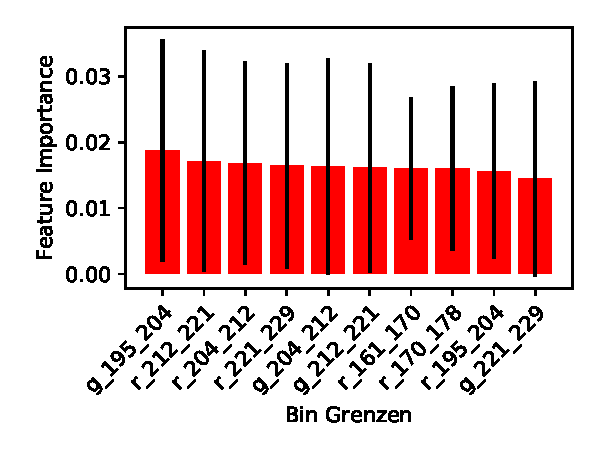
\includegraphics[width=0.5\textwidth]{./pictures/train_rf.pdf}
		\vspace{-1.4cm}
		\caption{Feature Importance des Random Forest.}
		\vspace{-1.4cm}
		\label{fig:}
\end{wrapfigure}
Für das Training des Random Forest können mehrere Parameter variiert werden.
Neben der maximalen Tiefe, der Anzahl an gezogenen Features pro Baum, kann die 
Anzahl an Entscheidungsbäumen variiert werden.
Da die Methode des Random Forest durch eine hohe Anzahl an Bäumen gegen 
Overfitting geschützt werden kann, werden die Tiefen der Bäume nicht weiter
beschränkt und die Anzahl an gezogenen Features nicht weiter optimiert.
Des Weiteren ist der histogrammierte Datensatz mit 30 bins pro Farbkanal für
maschinellen Lern Algorithmen sehr niederdimensional.
Bemerkenswert ist, dass der mit den angewendeten Farbschnitten Datensatz trainierte Forest die
Blauwerte verhältnismäßig geringer als die roten und grünen Bins gewichtet.
Durch das Trainieren auf den grünen und roten Werten, lernt der Random Forest
augenscheinlich ob der Himmel eher blaulich oder grau erscheint, da bei
Grauwerten alle Farbkanäle etwa gleich Groß sind.

\subsection{Convolution Neuronal Network}%
\label{sub:convolution_neuronal_network}

Die Optimierung des Netzes steht unter der Prämisse die Architektur des Netzes
so einfach wie Möglich zu halten, dass die ACC maximal wird und die Parameteranzahl, welche 
mit der Auswertungszeit korrelieren kann, gering bleibt. 
Beim Training mit der \texttt{categorical\_crossentropy} als Validation Loss stellt sich 
wider erwarten heraus, dass der Validation Loss bereits nach wenigen
Trainingsschritten wieder steigt, wohingegen die Accuracy noch 
signifikant steigt.
Dies liegt daran, wenn zum Beispiel bei dem wahren Label $A$ der 
Datensatz das Label $B$ hat. 
\begin{equation}
		H(p,q) = -\sum_x p(x) \log q(x)
\end{equation}
Somit wird die Wahrscheinlichkeit $q(B)$, die ein trainiertes Netz für die 
falsch klassifizierte Klasse klein und die Kreuzentropie groß.
Dies hat zur Folge, dass die Kreuzentropie bei Datensätzen mit einem Mismatch
bei der Validierung für hohe ACC nicht abnimmt, sondern schnell groß wird.
Das Übertraining kann durch eine Loss Funktion, welche nicht so sensibel auf
Mismatch ist, verringert werden. 
Dies ist beispielsweise für die in der Analyse verwendete \texttt{logcosh} der
Fall. 
Sie ähnelt für kleine Werte dem mittleren Quadratischen Fehler und nimmt für
große Werte einen linearen Zusammenhang an.
Desweiteren wird im Rahmen der Möglichkeiten versucht den Mismatch der Daten 
zu minimieren.

\begin{figure}[h]
		\centering
		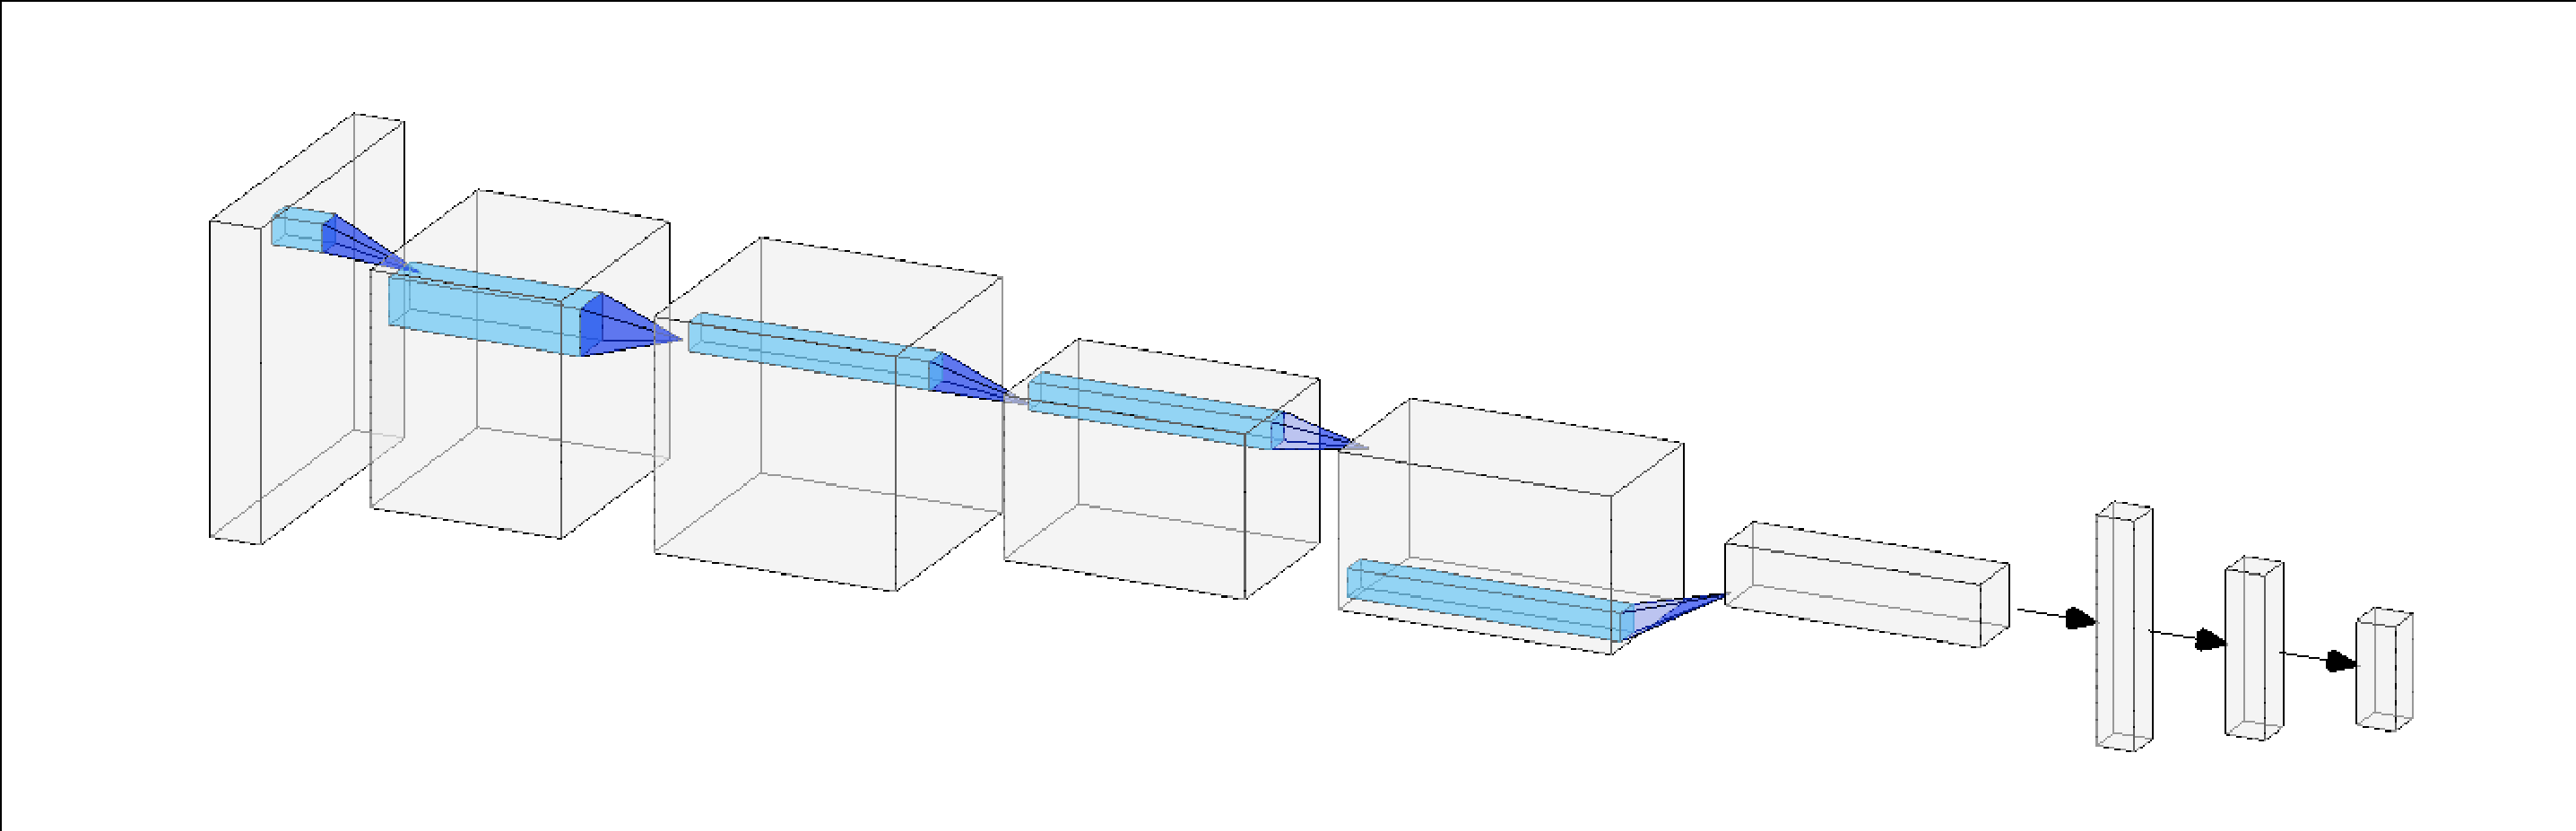
\includegraphics[width=0.8\textwidth]{pictures/architecture.pdf}
		\caption{Skizze der verwendeten Architektur des CNN \cite{nnsvg}}
		\label{fig:}
\end{figure}
Als Architektur wird zunächst eine \texttt{AveragePooling2D} Schicht mit einer
\texttt{poolsize} von \texttt{(3,4)} gewählt, um die Dimesonalität des Bildes zu verringern.
Dabei fiel die Wahl gegen die \texttt{MaxPooling2D} Schicht, da durch das 
Mitteln der Pixel deren Rauschen verringert werden kann.
Anschließend folgen sechs \texttt{Conv2D} Schichten, die der Faltung des Bildes
dienen. 
Die erste Convolutionschicht besitzt ein Schrittweite von \texttt{strides =
(3,3)}, was ebenso der Dimensionsreduktion dient.
Zwischen der zweiten und dritten Convolution-Schicht wird mittels
\texttt{MaxPooling2d} die Dimesonalität weiter verringert. 
Im Anschluss folgen nach der letzten \texttt{Conv2D} Schicht eine weitere
\texttt{MaxPooling2D} Schicht, bevor die Daten geflattet werden.
Beim \texttt{Flatten} wird aus einem hochdimensionalen Vektor ein flacher Vektor
mit der gleichen Anzahl an Einträgen.
Dieser kann von zwei aufeinanderfolgenden \texttt{Dense} Schichten verarbeitet
werden.
Bei einer \texttt{Dense} Schicht $i$ wird der flache Outpuvektor $x_i$ mit den
Gewichten $w_\text{ij}$ multipliziert, welche die Verbindung zur Folgeschicht
$j$ herstellen.
Diese werden durch jeweils eine \texttt{Dropout} und \texttt{GaussianNoise}- 
Schicht regularisiert. 
Dabei dient die \texttt{Dropout}- dazu die Gewichte $w_\text{ij}$ ausgeglichen
zu halten  
und die \texttt{Noise}-Schicht zu gewährleisten, dass diese klein sind.
Abschließend folgt eine \texttt{Dense}-Schicht mit der Anzahl an Neuronen der
Zielklassen.
Für die \texttt{kernel} der \texttt{Conv2D} sowie die \texttt{Dense}
Schichten wird die \texttt{relu} Funktion als Aktivierungsfunktion
genutzt.
Für die letzte Schicht wird die \texttt{sigmoid} Funktion verwendet, um die
Voraussagen glatt zu machen und auf eins zu normieren.
